\section{Modelado de sistemas}
\label{sec:modelado_de_sistemas}

El modelado de sistemas y de relaciones entre variables es una tarea fundamental en múltiples áreas de la ingeniería y la ciencia. Un sistema puede definirse como una relación funcional entre variables de entrada $x$ y salida $y$, donde la salida es una función de las entradas $y = f(x)$, como se muestra en la \reffig{system}.

\begin{figure}[H]
    \centering
    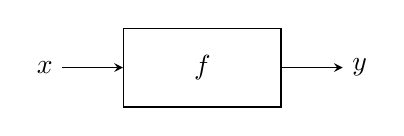
\begin{tikzpicture}
        \node (input) at (0, 0) [] {$x$};
        \node (output) at (4, 0) [] {$y$};
        \node[rectangle,, draw, minimum width=2cm, minimum height=1cm] (system) at (2, 0) {$f$};
        \draw[-stealth] (input) -- (system);
        \draw[-stealth] (system) -- (output);
    \end{tikzpicture}
    \caption{Sistema a modelar.}
    \label{fig:system}
\end{figure}

En este contexto, se busca aproximar la relación $y = f(x)$ mediante un modelo $\hat{f}$, con parámetros $\theta$, que permita estimar la salida $\hat{y}$ a partir de la entrada $x$, como se muestra en la \refeq{system_approximation} y la \reffig{system_model}.

\begin{equation}
    \label{eq:system_approximation}
    \hat{y} = \hat{f}(x; \theta) \approx f(x)
\end{equation}

\begin{figure}[H]
    \centering
    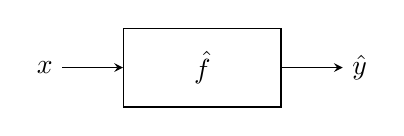
\begin{tikzpicture}
        \node (input) at (0, 0) [] {$x$};
        \node (output) at (4, 0) [] {$\hat{y}$};
        \node[rectangle,, draw, minimum width=2cm, minimum height=1cm] (system) at (2, 0) {$\hat{f}$};
        \draw[-stealth] (input) -- (system);
        \draw[-stealth] (system) -- (output);
    \end{tikzpicture}
    \caption{Modelo del sistema.}
    \label{fig:system_model}
\end{figure}

Con este objetivo, se define un problema de optimización a partir de una función de costo $L$ que mide el error entre la salida real $y$ y la salida estimada $\hat{y}$. A continuación, se buscan los parámetros $\theta$ que minimicen la función de costo $L(y, \hat{y})$. Generalmente, la función de costo incluye términos adicionales independientes del error, por ejemplo, penalizaciones para desalentar comportamientos no deseados del modelo \cite{Ng2004}.

En cuanto al tipo de salida, se distinguen dos clases de problemas de modelado: regresión y clasificación. La diferencia radica en el espacio de salida $y$. En los problemas de regresión, la variable de salida es continua, mientras que en los problemas de clasificación, la variable de salida es discreta y representa categorías o clases. Además de las funciones de costo, es importante seleccionar métricas de evaluación adecuadas para cada tipo de problema, que permitan cuantificar el desempeño del modelo en función de los objetivos específicos del mismo; dichas métricas se detallan en la sección \ref{sec:metricas}.

El proceso de encontrar los parámetros óptimos $\theta$ se denomina entrenamiento. Existen casos en los que se dispone de soluciones cerradas que pueden calcularse analíticamente. Sin embargo, en la mayoría de los problemas se emplean métodos numéricos iterativos para aproximar la solución óptima, dado que las soluciones cerradas son poco frecuentes en aplicaciones reales \cite{e23081012}.

Para llevar a cabo este proceso de entrenamiento, se requiere un conjunto de datos de entrada y salida conocidos (etiquetados) $\left(x_i, y_i\right)$, denominado conjunto de entrenamiento (o \textit{dataset} en inglés). Este tipo de aprendizaje se denomina aprendizaje supervisado, ya que estima una función a partir de datos etiquetados.

\subsection{Gradiente descendiente}
\label{sec:gradiente_descendiente}

El método iterativo más utilizado para ajustar los parámetros es el descenso por gradiente, que consiste en actualizar los parámetros en la dirección contraria al gradiente de la función de costo ($\nabla_{\theta} L(y, \hat{y})$), es decir, en la dirección que reduce el error \cite{9603742}. La actualización de los parámetros se realiza como se muestra en la ecuación \ref{eq:gradient_descent}, donde $\eta$ es la tasa de aprendizaje, que determina el tamaño del paso en cada iteración.

\begin{equation}
    \label{eq:gradient_descent}
    \theta_{n+1} = \theta_n - \eta \nabla_{\theta} L(y, \hat{y})
\end{equation}

Una variante de este algoritmo es el descenso por gradiente estocástico (de ahora en adelante SGD, por sus siglas en inglés de \textit{Stochastic Gradient Descent}), que utiliza un subconjunto aleatorio de los datos de entrenamiento en cada iteración para calcular el gradiente; véase la \refeq{sgd}. Esto reduce el costo computacional y puede ayudar a escapar de mínimos locales. Aunque introduce más ruido en el proceso de optimización, puede acelerar la convergencia \cite{robbins1951stochastic}.

\begin{equation}
    \label{eq:sgd}
    \theta_{n+1} = \theta_n - \eta \nabla_{\theta} L(y_i, \hat{y}_i)
\end{equation}

\subsection{Regresión lineal}
\label{sec:regresion_lineal}
El modelo de regresión lineal es uno de los modelos más simples y ampliamente utilizados en el aprendizaje supervisado \cite{Hastie2009}. Este modelo provee una estimación de una variable continua $y$ a partir de una variable independiente $x$, cuya relación se modela con una recta, como se muestra en la \refeq{linear_regression}.

\begin{equation}
    \label{eq:linear_regression}
    \hat{y} = \theta_0 + \theta_1 x
\end{equation}

Para ello, el objetivo es ajustar los parámetros $\theta_0$, $\theta_1$ que minimicen alguna métrica de error, definida por una función de costo $L$. En el caso de la regresión lineal, la función de costo utilizada comúnmente es el error cuadrático medio (o MSE por sus siglas en inglés \textit{Mean Squared Error}). Además, si se extrapola este modelo a un problema multivariable, la \refeq{linear_regression} se puede expresar como se muestra en la \refeq{linear_regression_multivariable}.

\begin{equation}
    \label{eq:linear_regression_multivariable}
    \hat{y} = \theta_0 + \sum_{j=1}^{m} \theta_j x_j
\end{equation}

En consecuencia, se buscan los valores de $\theta_0$, $\theta_1$, ..., $\theta_m$ que minimicen la función de costo definida en la \refeq{mse}. Para ello, se utiliza un conjunto de datos de tamaño $n$, donde $\mathbf{y}$ es el vector de salidas reales y $\hat{\mathbf{y}}$ es el vector de salidas estimadas por el modelo para las entradas correspondientes $\mathbf{X}$.

\begin{equation}
    \label{eq:mse}
    L(\mathbf{y}, \hat{\mathbf{y}}) = \frac{1}{n} \sum_{i=1}^{n} \left(y_i - \hat{y}_i\right)^2
\end{equation}

Para este problema particular, es posible deducir analíticamente los valores de $\mathbf{\theta}$ que minimizan la función de costo. Para esto, se deriva la función de costo con respecto a los parámetros $\frac{\partial L(\mathbf{y}, \hat{\mathbf{y}})}{\partial \mathbf{\theta}}$ y se iguala a cero. Al realizar esto, se obtiene la fórmula conocida como OLS (por sus siglas en inglés \textit{Ordinary Least Squares}), que permite calcular los parámetros óptimos de manera directa, como se muestra en la \refeq{ols}, donde $\mathbf{X}$ es la matriz de características, $\mathbf{\theta}$ es el vector de parámetros, y $\mathbf{y}$ es el vector de salidas reales, como se muestra en la \refeq{ols_matrices}.

\begin{equation}
    \label{eq:ols}
        \theta = \left(X^T X\right)^{-1} X^T y
\end{equation}

\begin{equation}
    \label{eq:ols_matrices}
      X =
        \begin{bmatrix}
        1 & x_{1,1} & x_{2,1} & \dots & x_{n,1} \\
        1 & x_{1,2} & x_{2,2} & \dots & x_{n,2} \\
        \vdots & \vdots & \vdots & \dots & \vdots \\
        1 & x_{1,m} & x_{2,m} & \dots & x_{n,m}
        \end{bmatrix}
      \quad \quad
      \theta =
        \begin{bmatrix}
          \theta_0 \\ \theta_1 \\ \theta_2 \\ \dots \\ \theta_n
        \end{bmatrix}
      \quad \quad
      y = \begin{bmatrix} y_1 \\ y_2 \\ \vdots \\ y_m \end{bmatrix}
    \end{equation}


Por lo tanto, este es un caso con solución cerrada, ya que permite calcular los parámetros óptimos de manera directa sin necesidad de utilizar métodos iterativos como el descenso por gradiente.

A modo de ilustración, el resultado de aplicar este modelo a un conjunto de datos se muestra en la \reffig{linear_regression}, donde se observa la línea de regresión ajustada a los datos, así como los errores entre las predicciones del modelo y los datos reales.

\defaultfigurecustomsize{regression/linear_regression.png}{Regresión Lineal.}{linear_regression}{1.1}

\subsection{Regresión logística}
\label{sec:regresion_logistica}

El modelo de regresión logística se utiliza en problemas de clasificación binaria. Estima la probabilidad de que una observación pertenezca a una clase mediante la función sigmoide \cite{Hosmer2013}, como se muestra en la \refeq{logistic_regression}.

\begin{equation}
    \label{eq:logistic_regression}
    \hat{y} = \mathbb{P}\left(y=1 \mid x\right)  = \frac{1}{1 + e^{-\left(\theta_0 + \sum_{j=1}^{m} \theta_j x_j\right)}}
\end{equation}

El valor de salida $\hat{y}$ pertenece al intervalo $(0, 1)$ y representa la probabilidad de que la observación pertenezca a la clase 1. En la práctica, se utiliza un umbral (comúnmente $0.5$). Si $\hat{y} \geq 0.5$, la observación se asigna a la clase 1; en caso contrario, a la clase 0. Véase la \reffig{logistic_regression}.

\defaultfigurecustomsize{regression/logistic_regression.png}{Regresión Logística.}{logistic_regression}{1.1}

En este modelo, la función de costo se define a partir de la verosimilitud. Bajo la hipótesis de independencia de las observaciones, la verosimilitud mide cuán probable resulta observar los datos dados los parámetros del modelo y se expresa como en la \refeq{likelihood} para una muestra de tamaño $n$.

\begin{equation}
    \label{eq:likelihood}
      V(\theta) = \prod_{i=1}^{n} \mathbb{P}(y_i \mid x_i)
\end{equation}

donde $\mathbb{P}(y_i \mid x_i)$ es la probabilidad de observar la clase $y_i$ dado el vector de características $x_i$. Por conveniencia computacional, se trabaja con el logaritmo de la función de verosimilitud, conocido como log-verosimilitud, que convierte el producto en una suma, como se muestra en la \refeq{log_likelihood}.

\begin{equation}
    \label{eq:log_likelihood}
      \ell(\theta) = \sum_{i=1}^{n} \left[ y_i \log(\mathbb{P}(y_i \mid x_i)) + (1 - y_i) \log(1 - \mathbb{P}(y_i \mid x_i)) \right]
\end{equation}

En consecuencia, la función de costo se define como el negativo de la log-verosimilitud; por lo tanto, el problema se plantea como la minimización de dicha función (equivalente a maximizar la log-verosimilitud) con respecto a los parámetros $\theta$. Dado que no existe una solución cerrada para este problema, se emplean métodos numéricos iterativos; en particular, el descenso por gradiente permite aproximar los parámetros que maximizan la verosimilitud.

\TODO{Revisar esta ultima parte}
En el caso de problemas con clasificación multiclase, se suele utilizar la función de costo de entropía cruzada generalizada (\textit{categorical cross-entropy} en inglés) cuya ecuación se muestra en la \refeq{categorical_cross_entropy} y la función de activación \textit{softmax}, cuya ecuación se muestra en la \refeq{softmax}, para modelar las probabilidades de pertenencia a cada clase.

\begin{equation}
    \label{eq:categorical_cross_entropy}
    L(\mathbf{y}, \hat{\mathbf{y}}) = - \sum_{i=1}^{n} \sum_{c=1}^{C} y_{i,c} \log(\hat{y}_{i,c})
\end{equation}

\begin{equation}
    \label{eq:softmax}
    \hat{y}_{i,c} = \frac{e^{z_{i,c}}}{\sum_{k=1}^{C} e^{z_{i,k}}}
\end{equation}

donde $C$ es el número de clases, $y_{i,c}$ es una variable indicadora que vale 1 si la observación $i$ pertenece a la clase $c$ y 0 en caso contrario, e $\hat{y}_{i,c}$ es la probabilidad estimada de que la observación $i$ pertenezca a la clase $c$, calculada mediante la función \textit{softmax} aplicada a los logits $z_{i,c}$.
